\documentclass{article}
\usepackage[utf8]{inputenc}
\usepackage{amsmath}
\usepackage{amsfonts}
\usepackage{appendix}
\usepackage{graphicx}

\title{The n-Volume Formula}
\author{Jack Hudson}
\date{September 2020}

% Write cylinder and cone volumes
% Write sphere surfaces and volumes
% 

\begin{document}

\maketitle

\[
\int_S \star \sqrt{f^{\star}g}
\]

\begin{abstract}
    
\end{abstract}

\section{Introduction}


\newpage
\tableofcontents
\newpage

\section{Deriving the Generalized n-Volume Formula}
\subsection{The Generalized Volume Element}
For any given volume, its n-volume\footnote{The n-volume is the generalized volume for n-dimensions. A 1-volume is a length, a 2-volume a surface area, and a 3-volume a volume. In general, an n-volume describes the size of a surface.} is given by $\int_S dV$, where $S$ is the domain of surface, and $dV$ is the n-volume element of the space. For any coordinate system, the volume element is given by $\sqrt{det(\eta)}$, followed by a chain of coordinate differentials for each coordinate describing a unique point in the volume. Here, $\eta$ is the metric of the space, which is the Minkowski Metric, as we will assume space to be flat for now.

In order to multiply by all coordinate differentials, the language of differential forms can be taken advantage of. Because $\sqrt{det(\eta)}$ is a pure function, it is in effect a 0-form. Applying the Hodge Star Operator to it, then, will yield its D-form twin, where D is the number of dimensions of the surface. For a three-dimensional surface parameterized by the coordinates $(x,y,z)$, the generalized volume element is then given by
\[
\star \sqrt{det(\eta)} = \sqrt{det(\eta)} dx \wedge dy \wedge dz
\]
and so the volume occupied by this surface is given by
\[
\int\int\int_S \sqrt{det(\eta)} dx \wedge dy \wedge dz
\]
where S is the domain of all three coordinates.

For a surface area or length, the same general formula can be applied. However, two or one coordinates would coordinatize the space, respectively, meaning that the integral would be over two or one coordinates.

\subsection{Pullback of the Metric Tensor}
The metric $\eta$ describes flat coordinates limiting it to only finding the volumes of rectangular prisms, the areas of rectangles, and the lengths of straight lines. However, any given surface has its own coordinates so long as it is parameterized. Therefore, the metric of that surface can be found via a pullback of the metric of the space the surface is embedded in. The simplest procedure for this is to find the space's coordinates in terms of the surface's coordinates, then to find the new metric in terms of the surface's coordinates. If the surface can be described by the mapping
\[
f(u,v): (x,y,z) \rightarrow (x(u,v), y(u,v), z(u,v))
\]
then the pullback of the metric $\eta$ by the mapping $f$ can be denoted $f^{\star}g$. In this example, a two dimensional surface is embedded in a three dimensional space. However, the pullback method to find the surface's metric will work for an any dimensional surface embedded in an any dimensional space.

For example, a surface parameterized by the coordinates $u$ and $v$ embedded in two dimensional Euclidean space would have coordinate differentials
\[
dx = \frac{\partial x}{\partial u}du + \frac{\partial x}{\partial v} dv, dy = \frac{\partial y}{\partial u}du + \frac{\partial y}{\partial v} dv
\]
Therefore, the metric:
\[
ds^2 = dx \otimes dx + dy \otimes dy
\]
Becomes
\[
ds^2 = (\frac{\partial x}{\partial u}du + \frac{\partial x}{\partial v} dv) \otimes (\frac{\partial x}{\partial u}du + \frac{\partial x}{\partial v} dv) + (\frac{\partial y}{\partial u}du + \frac{\partial y}{\partial v} dv) \otimes (\frac{\partial y}{\partial u}du + \frac{\partial y}{\partial v} dv)
\]
This new metric can now be directly plugged into the generalized n-volume formula:
\[
V = \int_S \star \sqrt{det(f^{\star}g)}
\]
\subsection{Procedure}
The procedure for utilizing the n-volume formula is relatively straightforward. It is as follows:
\begin{itemize}
    \item Find the parameterizing map.
    \item Find the coordinate differentials in terms of the parametric coordinates.
    \item Find the metric tensor in terms of the new coordinate differentials.
    \item Find the square root of the determinant of the metric tensor.
    \item Plug this into the integral and evaluate.
\end{itemize}
The remainder of this paper will be the process of following this procedure for a number of situations, and interpriting the results.

\newpage

\section{Flat Space}
The n-volume formula can be applied to a surface of any dimension embedded in a space of any dimension. However, in many trivial circumstances, it generalizes to simpler, common formulas. In the following section, the n-volume formula is used to derive some common geometric formulas.

\subsection{Reduction to the Arc Length Formula}
We will now set about to derive the arc length formula from the n-volume formula. Let $f(x)$ be an arbitrary function. As a map, this can be given by:
\[
f(t):(x,y)\rightarrow(x(t),y(t))
\]
Where $t=x$ and $y(t)=f(x)$. The 2D Minkowski metric is, of course:
\[
dx \otimes dx + dy \otimes dy
\]
Applying the pullback, the coordinate differentials are as follows:
\[
dx = \frac{\partial x}{\partial t} dt = dt, dy = \frac{\partial y}{\partial t} dt = f'(t) dt
\]
Therefore, the pullback of the metric by the function is
\[
dx \otimes dx + dy \otimes dy = dt \otimes dt + (f'(t))^2 dt \otimes dt = (1 + (f'(t))^2) dt \otimes dt
\]
The determinant of this metric is (as it is, as a matrix, a 1x1 matrix) simply $(1 + (f'(t))^2)$. Taking the square root of this yields $\sqrt{(1 + (f'(t))^2)}$. This is the $\sqrt{det(f^{\star}g)}$ part of the n-volume formula. Plugging it in yields
\[
\int_S \star \sqrt{(1 + (f'(t))^2)}
\]
The curve only has a singular dimension (t), making the Hodge star operator simply yield
\[
\int_S \sqrt{(1 + (f'(t))^2)}dt
\]
Because we have imposed $x=t$, we can replace $t$ by $x$ get the formula
\[
\int_{x_i}^{x_f} \sqrt{(1 + (f'(x))^2)}dx
\]
Here we have also added in the domain $S$. This formula is exactly the arc length formula!

QED

\subsubsection{Parametric Curves}
In the previous part, there was no motivation to set $x=t$. Let us now not make that assumption. The arbitrary map is now $f(t):(x,y)\rightarrow(x(t),y(t))$. The pullback of the metric now yields the coordinate differentials:
\[
dx = \frac{\partial x}{\partial t} dt, dy = \frac{\partial y}{t} dt
\]
The metric is then:
\[
dx \otimes dx + dy \otimes dy = (\frac{\partial x}{\partial t})^2 dt \otimes dt + (\frac{\partial y}{\partial t})^2 dt \otimes dt = ((\frac{\partial x}{\partial t})^2 + (\frac{\partial y}{\partial t})^2) dt \otimes dt
\]
The determinant of this metric is of course $(\frac{\partial x}{\partial t})^2 + (\frac{\partial y}{\partial t})^2$. Therefore, plugging that into the n-volume formula gives
\[
\int_S \star \sqrt{(\frac{\partial x}{\partial t})^2 + (\frac{\partial y}{\partial t})^2} = \int_{t_i}^{t_f} \sqrt{(\frac{\partial x}{\partial t})^2 + (\frac{\partial y}{\partial t})^2} dt
\]
Again, the domain $S$ has been inserted as the bounds of the integral. This is exactly the parametric arc length formula!

\subsection{Surface Areas of Three Dimensional Shapes}
The n-volume formula can be used to find surface areas as easily as it can be used to find lengths. It will now be applied to a number of common shapes in three dimensions in order to derive the formulas for their surface areas.

\subsubsection{The 2-Sphere}
A 2-sphere embedded in three dimensional space can be described by the parameterizing map $f(\theta,\phi):(x,y,z)\rightarrow(Rcos(\theta)sin(\phi),Rsin(\theta)sin(\phi),Rcos(\phi))$ for $\theta\in[0,\pi]$, $\phi\in[0,2\pi)$. Pulling back the metric by this parameterization yields the coordinate differentials:
\[
dx = \frac{\partial x}{\partial \theta} d\theta + \frac{\partial x}{\partial \phi} d\phi = -Rsin(\theta)sin(\phi) d\theta + Rcos(\theta)cos(\phi) d\phi
\]
\[
dy = \frac{\partial y}{\partial \theta} d\theta + \frac{\partial y}{\partial \phi} d\phi = Rcos(\theta)sin(\phi) d\theta + Rsin(\theta)cos(\phi) d\phi
\]
\[
dz = \frac{\partial z}{\partial \theta} d\theta + \frac{\partial z}{\partial \phi} d\phi = -Rsin(\phi) d\phi
\]
The full metric with pullback is extremely unwieldy, so the terms will be calculated individually.
\[
dx \otimes dx = R(-sin(\theta)sin(\phi) d\theta + cos(\theta)cos(\phi) d\phi) \otimes R(-sin(\theta)sin(\phi) d\theta + cos(\theta)cos(\phi) d\phi)
\]
\[
= R^2sin^2(\theta)sin^2(\phi) d\theta \otimes d\theta + R^2cos^2(\theta)cos^2(\phi) d\phi \otimes d\phi - 2R^2sin(\theta)sin(\phi)cos(\theta)cos(\phi) d\theta \otimes d\phi
\]
\[
dy \otimes dy = R(cos(\theta)sin(\phi) d\theta + sin(\theta)cos(\phi) d\phi) \otimes R(cos(\theta)sin(\phi) d\theta + sin(\theta)cos(\phi) d\phi)
\]
\[
= R^2cos^2(\theta)sin^2(\phi) d\theta \otimes d\theta + R^2sin^2(\theta)cos^2(\phi) d\phi \otimes d\phi + 2R^2cos(\theta)sin(\phi)sin(\theta)cos(\phi) d\theta \otimes d\phi
\]
\[
dz \otimes dz = R^2sin^2(\phi) d\phi \otimes d\phi
\]
Summing them all together and enacting some cancellations:
\[
R^2(sin^2(\theta)sin^2(\phi) + cos^2(\theta)sin^2(\phi)) d\theta \otimes d\theta + R^2(cos^2(\theta)cos^2(\phi) + sin^2(\theta)cos^2(\phi) + sin^2(\phi)) d\phi \otimes d\phi
\]
\[
= R^2sin^2(\phi) d\theta \otimes d\theta + R^2d\phi \otimes d\phi
\]
The determinant of this matrix is simply the product of the coefficients, as it is a diagonal metric:
\[
det(f^{\star}\eta) = R^4sin^2(\theta)
\]
Therefore the n-volume formula is
\[
\int_S \star R^2sin(\theta) = \int_S R^2sin(\theta) d\theta \wedge d\phi
\]
$S$ is the domain of the angles of the surface of a sphere, which we have already asserted to be $\theta\in[0,\pi]$, $\phi\in[0,2\pi)$. Therefore, the full integral is:
\[
\int_{0}^{2\pi}\int_{0}^{\pi}R^2sin(\theta) d\theta \wedge d\phi
\]
This integral will be computed explicitly, though going forward integral solutions will simply be given.
\[
2R^2\int_{0}^{2\pi}d\phi = 4\pi R^2
\]
Which is exactly the standard formula from geometry. QED

\subsubsection{The Torus}
The torus is defined by the following parameterization:
\[
f(\theta,\phi): (x,y,z) \rightarrow ((a cos(\theta)+b)cos(\phi), (a cos(\theta)+b)sin(\phi), a sin(\theta))
\]
\[
\theta, \phi \in [0, 2\pi)
\]
Here, $b$ is the larger radius of the torus, and $a$ is the smaller radius. The coordinate differentials are then:
\[
dx = (b cos\phi - a cos\phi sin\theta)d\theta - (a cos\theta+b)sin\phi d\phi
\]
\[
dy = (b cos\phi - a sin\phi sin\theta)d\theta + (a cos\theta + b)cos\phi d\phi
\]
\[
dz = a cos\theta d\theta
\]
Meaning:
\[
f^{\star}\eta = a^2 d\theta \otimes d\theta + (a cos \theta + b)^2 d\phi \otimes d\phi
\]
Giving an overall n-volume integral:
\[
\int_{0}^{2\pi}\int_{0}^{2\pi}(a^2 cos\theta + ab) d\theta \wedge d\phi = 4\pi^2ab
\]
This is, then, the formula for the surface area of the torus.

\subsubsection{The Cylinder}
The cylinder (more specifically, its side) is defined by the parameterizing map:
\[
f(\theta, z): (x,y,z) \rightarrow (R cos\theta, R sin\theta, z)
\]
The coordinate differentials are relatively straightforward:
\[
dx = -R sin(\theta) d\theta, dy = R cos(\theta) d\theta, dz = dz
\]
Therefore, the metric is:
\[
R^2 sin^2(\theta) d\theta \otimes d\theta + R^2 cos^2(\theta) d\theta \otimes d\theta + dz \otimes dz = R^2 d\theta \otimes d\theta + dz \otimes dz
\]
The n-volume formula is then simply
\[
\int_S \star R = \int_{0}^{h}\int_{0}^{2\pi} R d\theta \wedge dz = 2\pi Rh
\]
Here, $h$ is the height of the cylinder we are considering. This is, of course, the expected formula for its surface area.

\subsubsection{The Cone}
A cone with height $h$ and circular radius $R$ is parameterized by the map:
\[
R(\theta,t): (x,y,z) \rightarrow (Rt cos\theta, Rt sin\theta, h(1-t))
\]
\[
\theta \in [0, 2\pi), t \in [1, 0]
\]
Here, t is essentially the scale factor of the radius as one moves up the cone. As always, one must proceed by working out the coordinate differentials:
\[
dx = -Rt sin\theta d\theta + R cos\theta dt
\]
\[
dy = Rt cos\theta d\theta + R cos\theta dt
\]
\[
dz = -hdt
\]
\[
f^{\star}\eta = R^2 t^2 d\theta \otimes d\theta + (R^2 + h^2) dt \otimes dt
\]
The square root of the determinant of this metric is then:
\[
\sqrt{R^2t^2(R^2+h^2)} = Rt\sqrt{R^2+h^2}
\]
This $\sqrt{R^2+h^2}$ has a straightforward geometric interpretation: the slant height! It may be easier, then, to replace that radical with the slant height $l$, which will be used along with $R$ to differentiate between different cones. The n-volume formula is then:
\[
\int_S \star Rtl = \int_1^0\int_0^{2\pi} Rtl d\theta \wedge dt = -\int_0^1\int_0^{2\pi} Rtl d\theta \wedge dt
\]
This will, though, yield a negative area. Clearly, this is undesirable. The issue results from how the manifold (the cone) is oriented with respect to our coordinates. Reversing the orientation will cause the expression to pick up another negative sign, which will cancel the one existing, giving us the desired positive area. This can be done by simply reversing the order to differentiation, as the exterior product $\wedge$ is anti-symmetric. Therefore, the area is given by:
\[
\int_0^1\int_0^{2\pi} Rtl dt \wedge d\theta = \pi Rl
\]
As always, exactly as it should be.

\subsection{Volumes Contained in Three Dimensional Shapes}
\subsubsection{The Sphere}
The Minkowski Metric in spherical coordinates is given by:
\[
\eta = dr \otimes dr + r^2 d\theta \otimes d\theta + r^2 sin^2\theta d\phi \otimes d\phi
\]
In these coordinates, the parameterizing map for the interior of a sphere is:
\[
f(r, \theta, \phi):(r,\theta, \phi) \rightarrow (r, \theta, \phi)
\]
The pullback of the metric, then, is itself! This greatly simplifies calculations. The determinant of this metric is:
\[
r^2 sin^2 (\theta)
\]
Meaning that the n-volume formula yields:
\[
\int_S \star R^2 sin(\theta) = \int_{0}^{2\pi}\int_{0}^{\pi}\int_{0}^{R}R^2 sin(\theta) dr \wedge d\theta \wedge d\phi = \frac{4}{3}\pi R^3
\]
This is exactly the expected volume for a sphere.

\subsubsection{The Torus}
The interior of the torus is defined by:
\[
f(r,\theta,\phi): (x,y,z) \rightarrow ((r cos(\theta)+b)cos(\phi), (r cos(\theta)+b)sin(\phi), r sin(\theta))
\]
The coordinate differentials are:
\[
dx = cos(\theta)cos(\phi)dr - r sin(\theta) cos(\phi) d\theta - (r cos(\theta) + b) sin(\phi) d\phi
\]
\[
dy = cos(\theta)sin(\phi) dr - r sin(\theta) sin(\phi) d\theta + (r cos(\theta) + b) cos(\phi) d\phi
\]
\[
dz = sin(\theta) dr + r cos(\theta) d\theta
\]
Unfortunately, three dimensions can become rather complicated when dealing with cross-terms. However, the metric tensor is a rank-2 tensor, meaning that it can be represented as a matrix (specifically a 3x3 matrix). This will make it much simpler to see terms and how they cancel when we start adding together the coordinate differentials.
\[
dx \otimes dx =
\begin{bmatrix}
cos^2\theta cos^2\phi & -r sin\theta cos \theta cos^2 \phi & -(r cos\theta + b) cos\theta sin\phi cos\phi \\
-r cos\theta cos\theta cos^2\phi & r^2 sin^2\theta cos^2 \phi & r(r cos\theta + b)sin\theta sin\phi cos\phi \\
-(r cos\theta + b) cos\theta sin\phi cos\phi & r(r cos\theta + b)sin\theta sin\phi cos\phi & (r cos\theta + b) sin^2\phi
\end{bmatrix}
\]
\[
dy \otimes dy =
\begin{bmatrix}
cos^2\theta sin^2\phi & -r sin\theta cos \theta sin^2 \phi & (r cos\theta + b) cos\theta sin\phi cos\phi \\
-r sin\theta cos\theta sin^2\phi & r^2 sin^2\theta sin^2 \phi & -r(r cos\theta + b)sin\theta sin\phi cos\phi \\
(r cos\theta + b) cos\theta sin\phi cos\phi & -r(r cos\theta + b)sin\theta sin\phi cos\phi & (r cos\theta + b) cos^2\phi
\end{bmatrix}
\]
\[
dz \otimes dz =
\begin{bmatrix}
sin^2\theta & r sin\theta cos\theta & 0 \\
r sin\theta cos\theta & r^2 cos^2\theta & 0 \\
0 & 0 & 0
\end{bmatrix}
\]
These matrices are, evidently, extremely ugly. However, summing them leads to all of the off-diagonals cancelling, and many terms simplifying from simple trigonometric identities. The pulled-back metric is:
\[
f^{\star}\eta = \begin{bmatrix}
1 & 0 & 0 \\
0 & r^2 & 0 \\
0 & 0 & (r cos\theta + b)^2
\end{bmatrix}
\]
Therefore, the n-volume formula yields:
\[
\int_S \star (r^2 cos\theta + rb) = \int_0^{2\pi}\int_0^{2\pi}\int_0^{R}(r^2 cos\theta + rb) dr \wedge d\theta \wedge d\phi
\]
Splitting up this integral, it is easy to see that the first term will be 0. (This is because the integral of cosine from 0 to 2$\pi$ is 0.) Therefore, the integral simplifies to
\[
\int_0^{2\pi}\int_0^{2\pi}\int_0^{R} rb dr \wedge d\theta \wedge d\phi = 2\pi^2R^2b
\]
Which is exactly the volume within a torus.

\subsubsection{The Cylinder}
The parameterizing map for the interior of the cylinder is
\[
f(\rho, \theta, z): (x, y, z) \rightarrow (\rho cos \theta, \rho sin \theta, z)
\]
This makes the coordinate differentials:
\[
dx = cos(\theta) d\rho - \rho sin(\theta) d\theta, dy = sin(\theta) d\rho + \rho cos(\theta) d\theta, dz = dz
\]
\[
dx \otimes dx = cos^2 \theta d\rho \otimes d\rho + \rho^2 sin^2 \theta d\theta \otimes d\theta - 2\rho cos\theta sin\theta d\rho \otimes d\theta
\]
\[
dy \otimes dy = sin^2 \theta d\rho \otimes d\rho + \rho^2 cos^2 \theta d\theta \otimes d\theta + 2\rho cos\theta sin\theta d\rho \otimes d\theta
\]
\[
dz \otimes dz = dz \otimes dz
\]
Therefore, the metric is
\[
ds^2 = (cos^2 \theta + sin62 \theta) d\rho \otimes d\rho + (sin^2 \theta + cos^2 \theta) \rho^2 d\theta \otimes d\theta + dz \otimes dz = d\rho \otimes d\rho + \rho^2 d\theta \otimes d\theta + dz \otimes dz
\]
Finding the determinant is, then, simply $\rho^2$, meaning that the n-volume formula gives
\[
\int_S \star \rho = \int_0^h\int_0^{2\pi}\int_0^R \rho d\rho \wedge d\theta \wedge dz = \pi R^2h
\]
Exactly the expected volume of the cylinder.

\subsubsection{The Cone}
The parameterizing map for the interior of the cone is
\[
f(\rho, \theta, z): (x, y, z) \rightarrow ((1-\frac{z}{h})\rho cos \theta, (1-\frac{z}{h})\rho sin \theta, z)
\]
This gives the coordinate differentials
\[
dx = (1-\frac{z}{h}) cos\theta d\rho - (1-\frac{z}{h})\rho sin\theta d\theta - \frac{\rho}{h}cos\theta dz
\]
\[
dy = (1-\frac{z}{h}) sin\theta d\rho + (1-\frac{z}{h})\rho cos\theta d\theta - \frac{\rho}{h}sin\theta dz
\]
\[
dz = dz
\]
\[
dx \otimes dx = \begin{bmatrix}
 (1-\frac{z}{h})^2 cos^2 \theta &
  &
  \\
  &
 (1-\frac{z}{h})^2 \rho^2 sin^2 \theta &
  \\
  &
  &
 \frac{\rho^2}{h^2} cos^2 \theta
\end{bmatrix}
\]
\[
dy \otimes dy = \begin{bmatrix}
 (1-\frac{z}{h})^2 sin^2 \theta &
  &
  \\
  &
 (1-\frac{z}{h})^2 \rho^2 cos^2 \theta &
  \\
  &
  &
 \frac{\rho^2}{h^2} sin^2 \theta
\end{bmatrix}
\]
\[
dz \otimes dz = \begin{bmatrix}
 0 &   &   \\
   & 0 &   \\
   &   & 1 \\
\end{bmatrix}
\]
Because our coordinate system (cylindrical coordinates) is orthogonal, the off-diagonal terms of the metric must be 0, meaning that we can ignore the individual off-diagonal terms of the $dx \otimes dx$, $dy \otimes dy$, and $dz \otimes dz$ matrices. They may not be 0, but all three matrices must have off-diagonal terms that sum to zero, so explicitly writing them out would be useless.

Summing them now gives the overall metric:
\[
\eta = \begin{bmatrix}
 1-\frac{z}{h} & 0 & 0 \\
 0 & (1-\frac{z}{h}) \rho^2 & 0 \\
 0 & 0 & \frac{\rho^2}{h^2}
\end{bmatrix}
\]

\newpage

\section{Curved Space}
Now that the n-Volume formula has been proven to work in the simplest of cases, it can be applied to more exotic scenarios: curved spaces\footnote{See [Appendix A] for descriptions of the spaces we consider here}.

\subsection{Pullback of a Curved Metric}
The means by which a curved metric is pulled back is essentially identical to the flat (Euclidean) metric. First, the metric is explicitly identified:
\[
ds^2 = X(x,y,z) dx \otimes dx + Y(x,y,z) dy \otimes dy + Z(x,y,z) dz \otimes dz
\]
Then, the parameterizing map $f$ is also explicitly defined, as well as all of the parametrized coordinates. The coordinate differentials $dx$, $dy$, and $dz$ are then identified in terms of the parameterized coordiantes, and the metric is then found in terms of those coordinates. Finally, the metric is inserted into the n-volume formula, and all that remains to be done is the evaluation of the resulting integral.

\newpage
\subsection{Path Length}
\subsubsection{Standard Metric}
Many space-time metrics from General Relativity (specifically spherically symmetric ones) take the form
\[
ds^2 = -f(r) dt \otimes dt + f(r)^{-1} dr \otimes dr + r^2 d\Omega_2 \otimes d\Omega_2
\]
Because we are only considering the sizes of shapes, time is unchanging, reducing the standard metric to
\[
ds^2 = f(r)^{-1} dr \otimes dr + r^2 d\Omega_2 + d\Omega_2
\]
Because many metrics take this form, it is a much more reasonable endeavor to work out the lengths, areas, and volumes of shapes in terms of any general $f(r)$, and then to simply insert the proper $f(r)$ for any particular space and evaluate, once the specific space is known. Below is a table of $f(r)$ expressions and the spaces they represent:
\[
\begin{tabular}{|c|c|}
\hline
    Expression & Space \\ \hline
    $1$ & Minkowski/Euclidean Space \\ \hline
    $1 - \frac{2GM}{r}$ & Schwartzchild Space \\ \hline
    $1 - \frac{r^2}{\alpha^2}$ & de Sitter Space \\ \hline
    $1 + \frac{r^2}{\alpha^2}$ & Anti-de Sitter Space \\ \hline
\end{tabular}
\]

Now, to find the path length. A general path in polar coordinates can be represented by the map:
\[
\mu(t): (r, \theta, \phi) \rightarrow (R(t), \Theta(t), \Phi(t))
\]
Here, $\mu$ represents the map, as $f$ is already taken, as part of the metric. Speaking of, the metric is the standard metric
\[
ds^2 = \frac{1}{f(r)} dr \otimes dr + r^2 d\Omega_2 \otimes \Omega_2
\]
The coordinate differentials are the straightforward:
\[
dx = (R'(t))^2 dt, dy = (\Theta'(t))^2 dt, dz = (\Phi'(t))^2 dt
\]
Therefore, the metric is:
\[
ds^2 = (\frac{1}{f(r)}(R'(t))^2 + r^2 (\Theta'(t))^2 + r^2 sin^2(\Theta(t))(\Phi'(t))^2) dt \otimes dt
\]
This has only one element as a matrix, yielding a straightforward determinant. The n-volume formula is therefore:
\[
\int_S \sqrt{\frac{1}{f(r)}(R'(t))^2 + r^2 (\Theta'(t))^2 + r^2 sin^2(\Theta(t))(\Phi'(t))^2} dt
\]
However, it is rare that a path is specified with angles as functions of time, except for very specific circumstances. Therefore, it is useful to convert now to Cartesian coordinates, via the definitions:
\[
r = \sqrt{x^2 + y^2 + z^2}, \theta = arctan(\frac{y}{x}), \phi = arctan(\frac{\sqrt{x^2 + y^2}}{z})
\]
Plugging these definitions into the formula whole, however, would result in a monstrously long expression, and so it is simply necessary to convert on a case-by-case basis. The generalized length formula we have now cannot be analyzed any further without specifying a particular spacial geometry.

\subsubsection{Schwartzschild Space}
The $f$ expression for Schwartzschild space is $1-\frac{2GM}{r}$. Inserting this into the standard metric path length formula yields:
\[
\int_S \sqrt{\frac{1}{1-\frac{2GM}{R(t)}}(R'(t))^2 + (R(t))^2 (\Theta'(t))^2 + (R(t))^2 sin^2(\Theta(t))(\Phi'(t))^2} dt
\]
It is difficult to see clearly how geometry is affected by this strange space. Therefore, two examples will be considered: the line $x+y=3GM$, and the circle with radius $3GM$. Recall that the Schwartzschild metric breaks down at radii closer than $2GM$, as that is the location of a singularity usually corresponding to the event horizon of a black hole. This means that any structure considered with this metric must lay outside of the event horizon, or else a different metric--the interior solution--would be needed.

First, for the line $x+y=3GM$. Using the parameterization $x=t$, we get:
\[
x=t, y=3GM-t, z=0
\]
Converting to spherical coordinates gives
\[
R(t) = \sqrt{t^2 + (3GM-t)^2}, R'(t) = \frac{2t - 3GM}{\sqrt{9G^2M^2 - 6GMt + 2t^2}}
\]
\[
\Theta(t) = arctan(\frac{3GM-t}{t}), \Theta'(t) = \frac{3GM}{9G^2m^2 - 6GM + 2t^2}
\]
\[
\Phi(t) = \frac{\pi}{2}, \Phi'(t) = 0
\]
For sake of simplification, we shall use the definition $\Delta(t) = R^2(t) = 9G^2M^2 - 6GMt + 2t^2$. Therefore, the path's length is:
\[
\int_S \sqrt{\frac{1}{1-\frac{2GM}{\sqrt{t^2 + (3GM-t)^2}}}
(\frac{(2t-3GM)^2}{\Delta(t)})
+\frac{9G^2M^2}{\Delta(t)}} dt
\]
This is difficult to analyze as it is, but graphing the length of the path as a function of $t$ (the x-distance along the path) yields:
\[
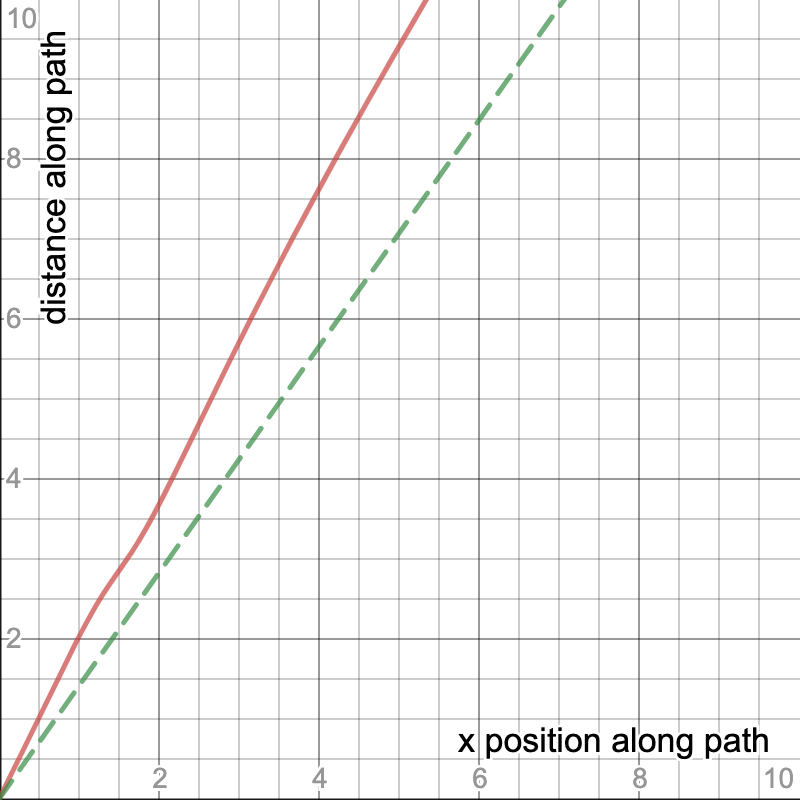
\includegraphics[scale=0.25]{schwartzchildpathlength.png}
\]
Here, all distances are measured in units where $MG$ is $1$. The dashed line is the path length in Euclidean space, for comparison. It is much easier to see graphically that Schwartzschild space appears to stretch out the path, proportionally to the distance from the singularity causing the curvature. This is somewhat intuitive within General Relativity, as the black hole modeled by the Schwartzschild metric would be seen as bending space due to its mass, which would stretch out the path.

As for the circle of radius $3GM$, its representation in spherical coordinates is
\[
R(t) = 3GM, R'(t) = 0
\]
\[
\Theta(t) = t, \Theta'(t) = 1
\]
\[
\Phi(t) = \frac{\pi}{2}, \Phi'(t) = 0
\]
The path length is, then:
\[
\int_0^{2\pi} \sqrt{\frac{1}{1-\frac{2GM}{3GM}}(0)^2 + (3GM)^2 (1)^2 + (3GM)^2 sin^2(t)(0)^2} dt
\]
The fact that both the radius and $\Phi(t)$ are constant cancels out two of the three terms in the radicand. Notice that because the radius is constant, $f(t)$ will be removed from the expression altogether. This means that the space simply does not affect the circumference of the circle. Finishing out the calculation yields:
\[
\int_0^{2\pi} \sqrt{(3GM)^2} dt = \int_0^{2\pi} 3GM dt = 6\pi GM
\]
This is exactly $2\pi R$, meaning that the curvature of space has no bearing on the circumference of the circle, even though straight lines through the space do have difference lengths than in the Euclidean limit.

\subsubsection{de Sitter Space}
de Sitter space has $f(r) = 1 - \frac{r^2}{\alpha^2}$. This gives a path length of
\[
\int_S \sqrt{\frac{1}{1 - \frac{r^2}{\alpha^2}}(R'(t))^2 + r^2 (\Theta'(t))^2 + r^2 sin^2(\Theta(t))(\Phi'(t))^2} dt
\]
Now, the path along the line $x+y = 3GM$ will be considered again\footnote{The circle has already been proven independent of curvature, so it will not be calculated again.}. The coordinates are, of course:
\[
R(t) = \sqrt{t^2 + (3GM-t)^2}, R'(t) = \frac{2t - 3GM}{\sqrt{9G^2M^2 - 6GMt + 2t^2}}
\]
\[
\Theta(t) = arctan(\frac{3GM-t}{t}), \Theta'(t) = \frac{3GM}{9G^2m^2 - 6GM + 2t^2}
\]
\[
\Phi(t) = \frac{\pi}{2}, \Phi'(t) = 0
\]
Giving the length
\[
\int_S \sqrt{\frac{1}{1-\frac{r^2}{\alpha^2}}
(\frac{(2t-3GM)^2}{\Delta(t)})
+ \frac{9G^2M^2}{\Delta(t)}} dt
\]
Again, this formula is not simple to analyze. However, graphing the length of the path gives:
\[
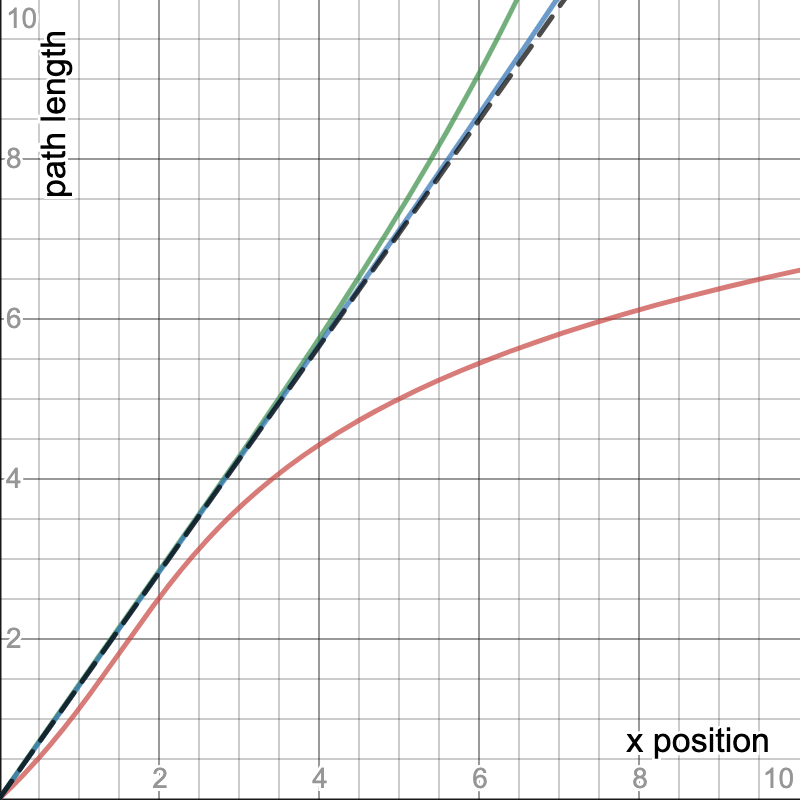
\includegraphics[scale=0.25]{desitterpathlength.png}
\]
Here, $\alpha=1$ is the rightmost curve (in red), $\alpha=10$ is the leftmost curve (in green), and $\alpha=100$ is the central curve (in blue). The black, dotted line is the Euclidean path length, for comparison. At lower values of $\alpha$, the path appears to be condensed, while for values, the path is stretched, as in Schwartzschild space. It can be seen clearly that for any $\alpha$, as the path gets shorter and shorter, the Euclidean approximation gets more adn more accurate. However, this is somewhat trivial, as it is true for any manifold, including de Sitter space. Graphing $\alpha$ values against the length of the path where $x \in [0, 3]$ allows some relationships to be seen more clearly.
\[
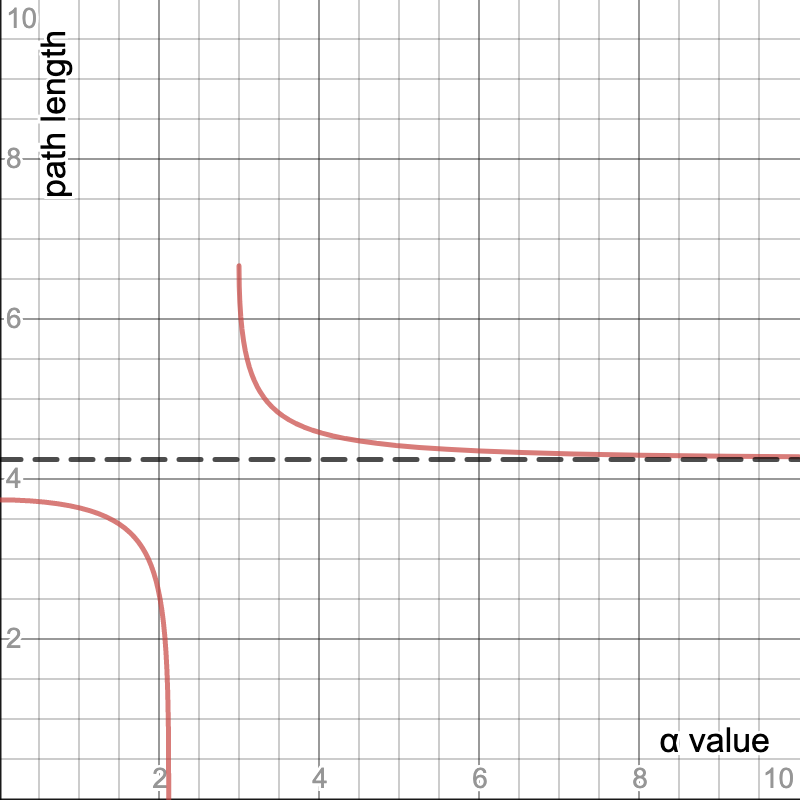
\includegraphics[scale=0.25]{desitterlength.png}
\]
This shows visually the connection between $\alpha$ and how the path is condensed or stretched. When $\alpha$ is below $3$, the path is shorter than it would be in flat space, while when $\alpha$ is above $3$, it is longer. For $\alpha=3$, the path length asymptotically diverges.

\subsubsection{anti-de Sitter Space}
Anti-de Sitter space has a similar $f(r)$ expression to de Sitter space: $f(r)=1+\frac{r^2}{\alpha^2}$. Again, the line $x+y=3GM$ will be considered. The path length is given by:
\[
\int_S \sqrt{\frac{1}{1+\frac{r^2}{\alpha^2}}
(\frac{(2t-3GM)^2}{\Delta(t)})
+ \frac{9G^2M^2}{\Delta(t)}} dt
\]
As always, we shall graph the path length as a function of $x$ position. It yields:
\[
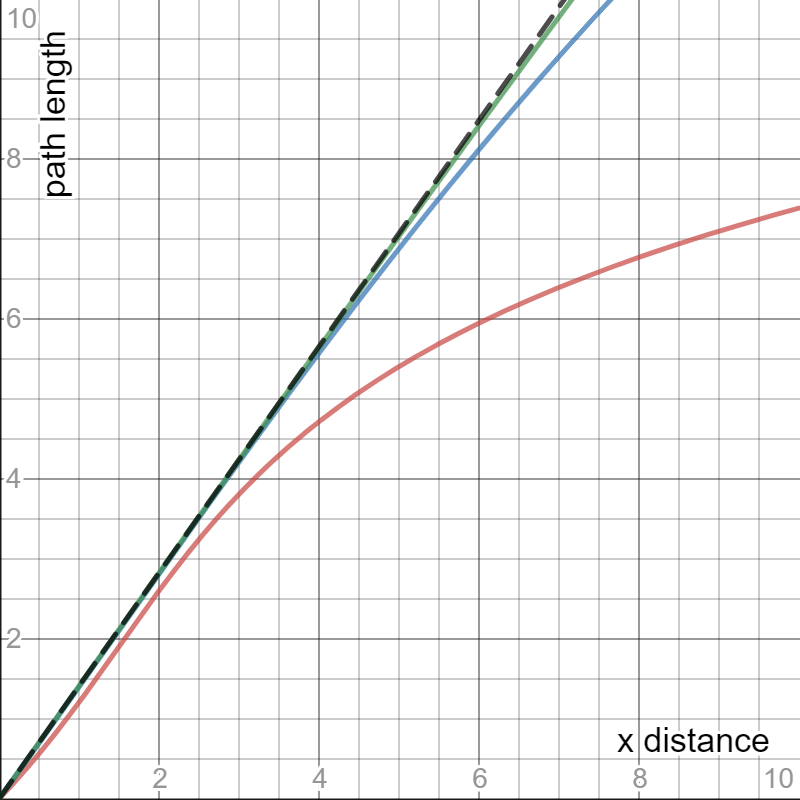
\includegraphics[scale=0.25]{antidesitterpathlength.png}
\]
Here, the rightmost curve (red), middle curve (blue), and leftmost curve (green) represent the path lengths when $\alpha$ is $1$, $10$, and $25$, respectively. Again, for path lengths, any value of $\alpha$ will be approximately Euclidean, as anti-de Sitter space is a manifold. Plotting the change in the path length as $\alpha$ increases gives
\[
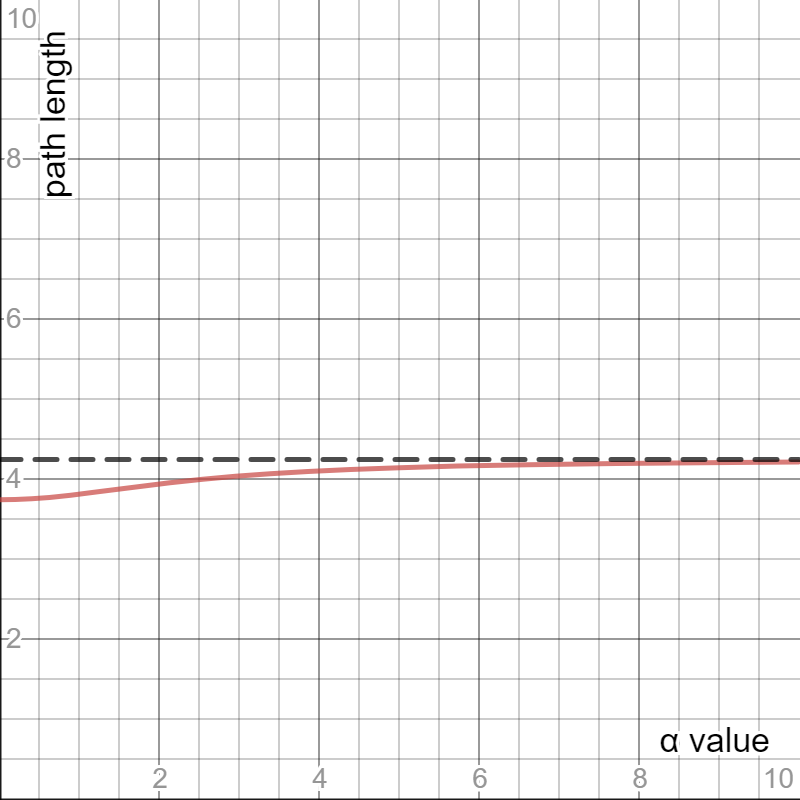
\includegraphics[scale=0.25]{antidesitterlength.png}
\]
This demonstrates clearly that anti-de Sitter space shrinks the path for any $\alpha$, but approaches the flat space value as $\alpha$ goes to infinity.


\newpage
\subsection{The Sphere and the Shell}
\subsubsection{Standard Metric}
The sphere's interior in spherical coordinates requires no paramterization, but its coordinates follow:
\[
r \in [0, R], \theta \in [0, \pi), \phi \in [0, 2\pi)
\]
The metric is, of course
\[
ds^2 = \frac{1}{f(r)} dr \otimes dr + r^2 d\Omega_2 \otimes d\Omega_2
\]
Finding the determinant, taking the square root, and combining everything into the n-volume formula yields:
\[
\int_0^{2\pi}\int_0^\pi\int_0^R \frac{r^2 sin\theta}{\sqrt{f(r)}} dr \wedge d\theta \wedge d\phi
\]
Switching the order of integration twice introduces two negative signs, which "cancel out", thereby giving
\[
\int_0^R\int_0^{2\pi}\int_0^\pi \frac{r^2 sin\theta}{\sqrt{f(r)}} d\theta \wedge d\phi \wedge dr
= 4 \pi \int_0^R \frac{r^2}{\sqrt{f(r)}} dr
\]
Which is as simplified as can be withing specifying a particular space.

The surface of the sphere, however, has no variation in the radius, and so its pulled-back metric is given by:
\[
ds^2 = r^2 d\Omega_2 \otimes d\Omega_2
\]
This has no dependence on $f(r)$, and so any space described by a standard metric will find the same value for the surface area of a sphere of any given radius.

\subsubsection{Schwartzschild Space}
For Schwartzschild Space, the volume of the sphere is given by
\[
4 \pi \int_0^R \frac{r^2}{\sqrt{1 - \frac{2GM}{r}}} dr
\]
However, the coordinate singularity at $r=2GM$ means that any manifold which contains that sphere will have a volume which asymptotically approaches infinity. Therefore, a sphere cannot be analyzed, but a shell can. The volume of this shell will be given by
\[
4 \pi \int_{R_L}^{R_G} \frac{r^2}{\sqrt{1 - \frac{2GM}{r}}} dr
\]
Here, $R_L$ is the lesser radius, and $R_G$ the greater radius. Taking the lesser radius to be $3GM$ and graphing the volume as a function of the greater radius yields:
\[
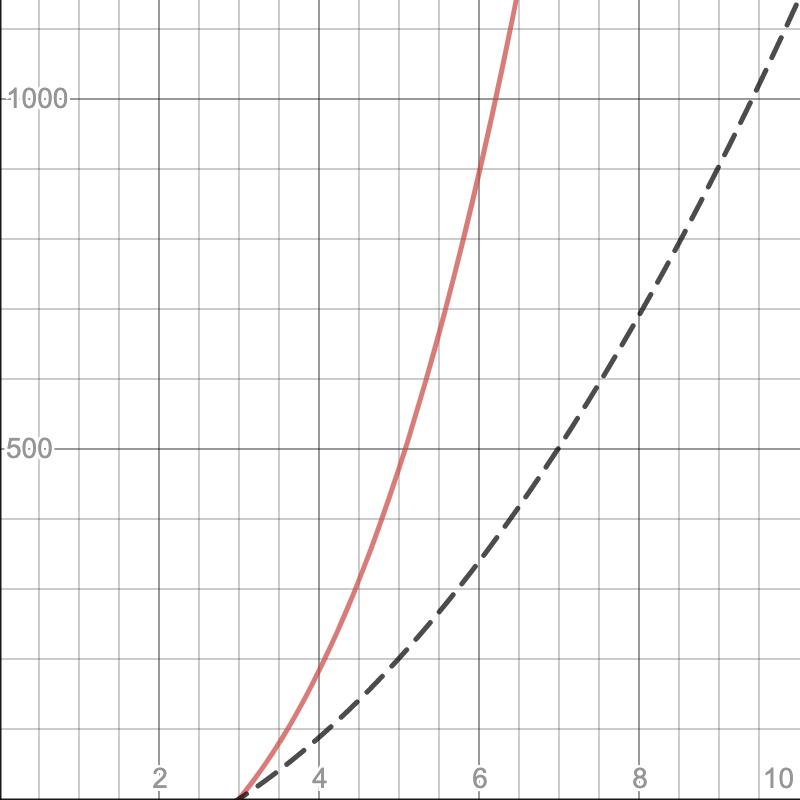
\includegraphics[scale=0.25]{schwartzschildsphere.png}
\]
The left curve (red) is the shell's volume in Schwartzschild space, graphed against the volume in flat space (dashed curve). As with the path length example, the Schwartzschild metric appears to stretch space.

\subsubsection{de Sitter Space}
The sphere volume in de Sitter space is instead
\[
4 \pi \int_0^R \frac{r^2}{\sqrt{1-\frac{r^2}{\alpha^2}}} dr
\]
There is no coordinate singularity in de Sitter space, and so the sphere can be safely considered, without needing to result to the shell. Plotting the volume as a function of the radius gives:
\[
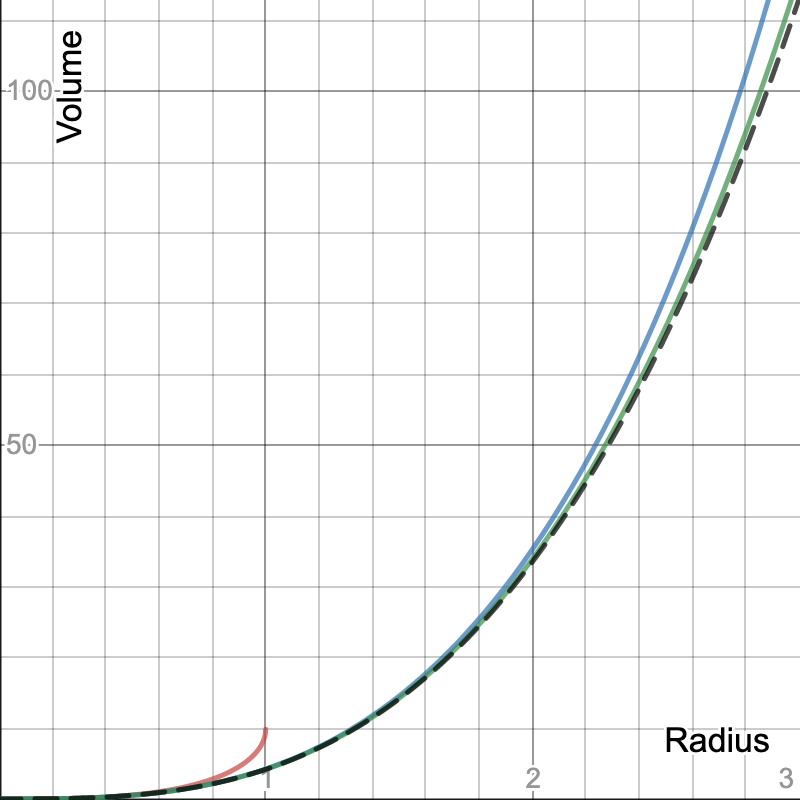
\includegraphics[scale=0.25]{desittersphere.png}
\]
The leftmost curve (red), middle curve (blue), and rightmost curve (green) represent the volume as a function of radius in de Sitter spaces with $\alpha$ set to $1$, $5$, and $10$, respectively. The maximum radius cutoffs correspond to boundaries of the space.

The volume as a function of $\alpha$ value is
\[
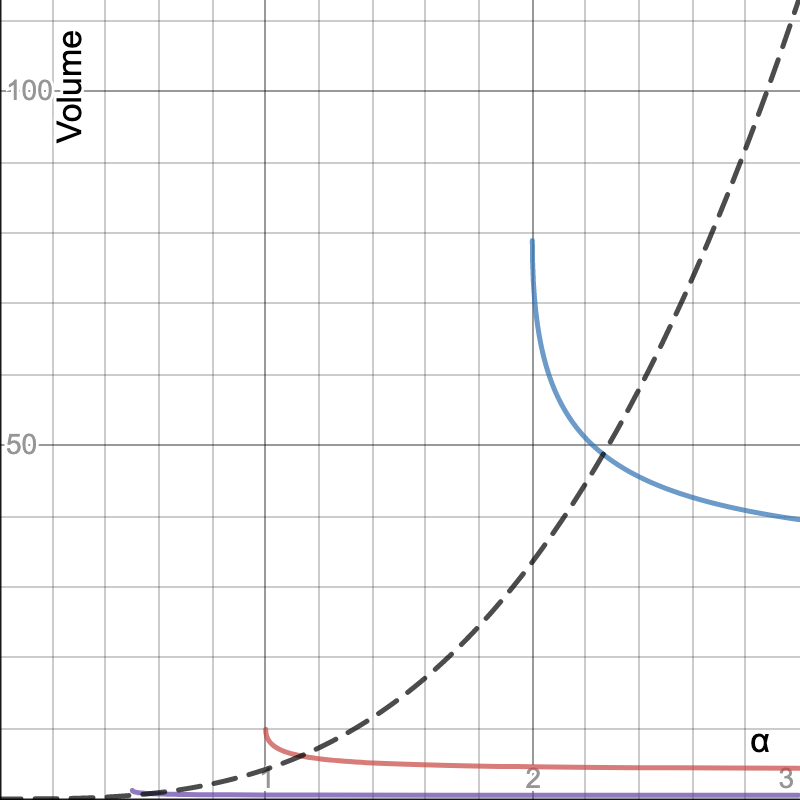
\includegraphics[scale=0.25]{desittersphere2.png}
\]

The bottom (purple), middle (red) and top (blue) curves correspond to spheres of radius $0.5$, $1$, and $2$, respectively. The graph makes it clear that the radius must be at least the $\alpha$ value, or else the volume is undefined.

\subsubsection{anti-de Sitter Space}
Anti-de Sitter space has the sphere volume
\[
4 \pi \int_{R_L}^{R_G} \frac{r^2}{\sqrt{1 + \frac{2GM}{r}}} dr
\]
As always, graphs will provide key insight into the behaviour of the space. First, the volume as a function of the radius for various $\alpha$ values.
\[
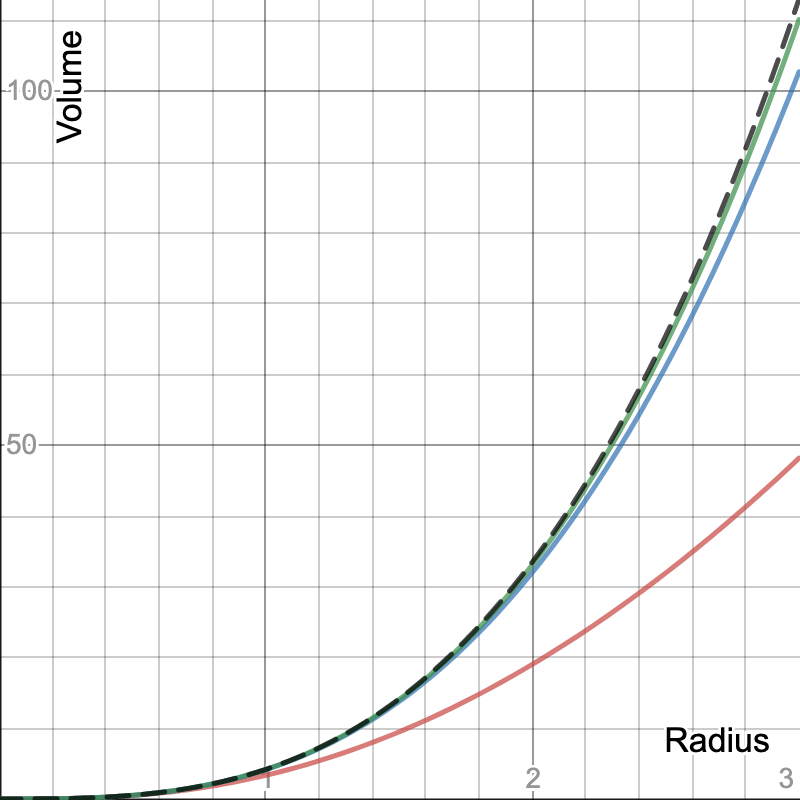
\includegraphics[scale=0.25]{antidesittersphere.png}
\]
As was seen with the path lengths, Anti-de Sitter space appears to shrink space, as compared to Euclidean space. The volume of the unit sphere as a function of $\alpha$ is plotted as
\[
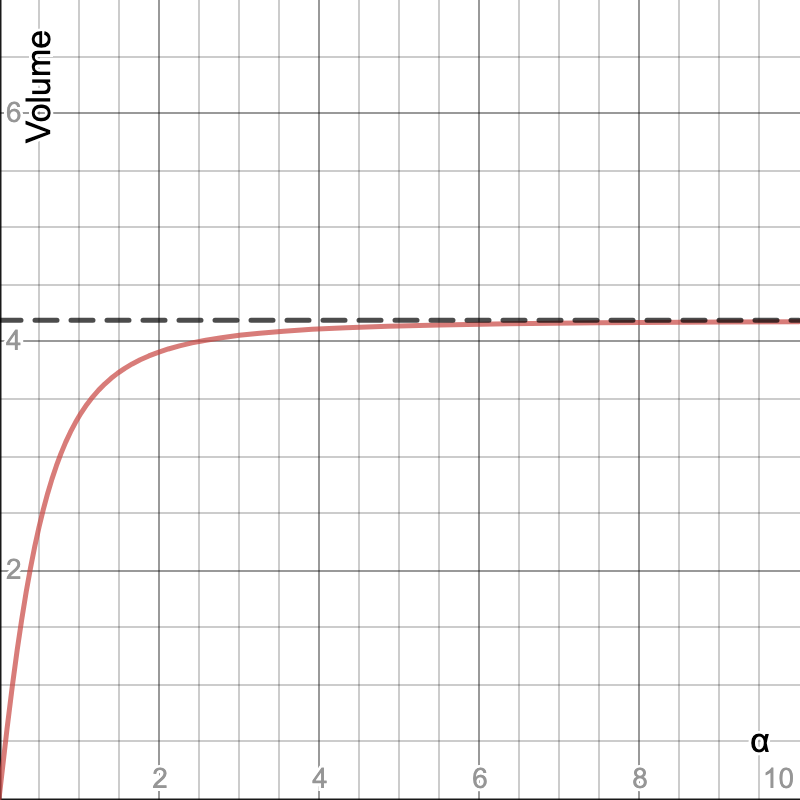
\includegraphics[scale=0.25]{antidesittersphere2.png}
\]
Clearly, the lower the $\alpha$ value, the more space shrinks, eventually compacting the volume of the unit sphere down to nothing. Likewise, as $\alpha$ increases in value, the space tends to Euclidean space.

\newpage
\subsection{The Cylinder}
\subsubsection{Standard Metric}
The parameterizing map for the surface of the cylinder (in spherical coordinates) is
\[
\mu(z, \Theta): (r, \theta, \phi) \rightarrow (\sqrt{R^2 + z^2}, \Theta, 0)
\]
Making the coordinate differentials:
\[
dr = \frac{z}{\sqrt{R^2+z^2}}dz, d\theta = d\Theta, d\phi = 0
\]
Therefore, the metric is
\[
ds^2 = \frac{1}{f(r)}\frac{R^2}{R^2+z^2} dz \otimes dz + (R^2 + z^2) d\Theta \otimes d\Theta
\]
The determinant of this metric, square-rooted, and plugged into the n-volume formula yields:
\[
\int_0^h\int_0^{2\pi} R\sqrt{\frac{1}{f(r)}}) dz \wedge d\Theta
\]

\subsubsection{Schwartzschild Space}
\subsubsection{de Sitter Space}
\subsubsection{anti-de Sitter Space}

\newpage
\subsection{The Cone}
\subsubsection{Standard Metric}
\subsubsection{Schwartzschild Space}
\subsubsection{de Sitter Space}
\subsubsection{anti-de Sitter Space}

\newpage
\section{Results}


\newpage
\appendix
\section{The Spaces Considered}
\subsection{Euclidean Space}
\subsection{Schwartzschild Space}
\subsection{de Sitter Space}
\subsection{Anti-de Sitter Space}

\end{document}
